% Uncomment for handout
%\def\HANDOUT{}


\ifdefined\HANDOUT
\documentclass[handout]{beamer}
\usepackage{pgfpages}
\pgfpagesuselayout{4 on 1}[letterpaper,landscape,border shrink=5mm]
\else
\documentclass{beamer}
\fi

\mode<presentation>
{
  \usetheme{Warsaw}
  \definecolor{sered}{rgb}{0.78, 0.06, 0.18}
  \definecolor{richblack}{rgb}{0.0, 0.0, 0.0}
  \setbeamercolor{structure}{fg=sered,bg=richblack}
  %\setbeamercovered{transparent}
}


\usepackage[english]{babel}
\usepackage[latin1]{inputenc}
\usepackage{times}
\usepackage[T1]{fontenc}
\usepackage{tikz}
\usepackage{graphicx}
\usepackage[export]{adjustbox}
\usepackage{fancyvrb}
\usepackage{amsmath}
\usepackage{amssymb}

\newcommand{\imagesource}[1]{{\centering\hfill\break\hbox{\scriptsize Image Source:\thinspace{\tiny\itshape #1}}\par}}
\newcommand{\image}[2]{%
        \begin{center}
        \includegraphics[max height = 0.55\textheight, max width = \textwidth]{images/#1}
        \linebreak
        
        {\tiny Image Source:\thinspace{\tiny #2}}
        \end{center}
}

\newenvironment{code}{%
 \VerbatimEnvironment
 \begin{adjustbox}{max width=\textwidth, max height=0.7\textheight}
 \begin{BVerbatim}
  }{
  \end{BVerbatim}
 \end{adjustbox}
}

\title{01 - Introduction to Tensor Analytics}


\author{Robert Lowe}

\institute[Southeast Missouri State University] % (optional, but mostly needed)
{
  Department of Computer Science\\
  Southeast Missouri State University
}

\date[]{}
\subject{}

\pgfdeclareimage[height=1.0cm]{university-logo}{images/semo-logo}
\logo{\pgfuseimage{university-logo}}



\AtBeginSection[]
{
  \begin{frame}<beamer>{Outline}
    \tableofcontents[currentsection]
  \end{frame}
}


\begin{document}

\begin{frame}
  \titlepage
\end{frame}



% Structuring a talk is a difficult task and the following structure
% may not be suitable. Here are some rules that apply for this
% solution: 

% - Exactly two or three sections (other than the summary).
% - At *most* three subsections per section.
% - Talk about 30s to 2min per frame. So there should be between about
%   15 and 30 frames, all told.

% - A conference audience is likely to know very little of what you
%   are going to talk about. So *simplify*!
% - In a 20min talk, getting the main ideas across is hard
%   enough. Leave out details, even if it means being less precise than
%   you think necessary.
% - If you omit details that are vital to the proof/implementation,
%   just say so once. Everybody will be happy with that.

\begin{frame}{Course Overview}
    \begin{columns}
    \column{0.5\textwidth}
    \begin{itemize}
        \item Means of Communication
        \begin{itemize}
            \item \href{https://semo.instructure.com/courses/8742}{Canvas}
            \item \href{https://teams.microsoft.com/l/team/19\%3aUpB3PjqRhBNybZmelVdPRJ8Y9d_-qosJxCWbuxIsaVE1\%40thread.tacv2/conversations?groupId=bd2ac44b-b270-4b10-8140-7708728805a9&tenantId=19d57598-97b0-442c-b74e-c855b0d87caf}{Microsoft Teams}
        \end{itemize}
        \item \href{https://semo.instructure.com/courses/8742/assignments/syllabus}{The Course Syllabus}
    \end{itemize}
    
    \column{0.5\textwidth}
    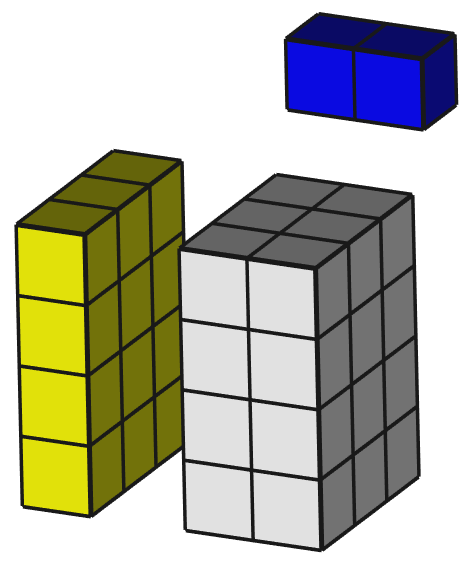
\includegraphics[max width=\textwidth]{images/tensor}
    \end{columns}
\end{frame}

\begin{frame}{Software}
    \begin{center}
    \href{https://www.python.org}{
\includegraphics[max width=0.5\textwidth, max height=0.4\textheight]{images/python}}
    \href{https://www.numpy.org}{
\includegraphics[max width=0.25\textwidth, max height=0.4\textheight]{images/numpy}}\newline
    \vspace{0.1\textheight}
    \newline
    \href{https://www.tensorflow.org}{
\includegraphics[max width=0.5\textwidth, max height=0.4\textheight]{images/tensorflow}}
    \end{center}
\end{frame}

\begin{frame}{Secondary Goals}
    \begin{columns}
    \column{0.5\textwidth}
    \begin{itemize}
        \item I want to establish a research group.
        \item I want you to join the research group.
        \item By bringing you up to speed with current tensor research, I want you to help me advance the state of the art!
        \item Let's publish some papers together!
    \end{itemize}
    \column{0.5\textwidth}
        \begin{center}
        
\includegraphics[max width=\textwidth, max height=0.65\textheight]{images/tensor-recruit}
        \end{center}
    \end{columns}
\end{frame}

\begin{frame}{What is Big Data?}
    \begin{itemize}
        \item Big in Terms of Cases $\longrightarrow$ Potential Over-fitting
        \item Big in Terms of Variables $\longrightarrow$ The Curse of Dimensionality
    \end{itemize}
\end{frame}

\begin{frame}{Example: Automatic Light}
    \begin{block}{Problem Statement}
        Suppose we have a light in a room, but we are too lazy to consistently use the light switch to turn it on and off.
        How might we automate our illumination needs?
    \end{block}
\end{frame}

\begin{frame}{The Curse of Dimensionality}
    \begin{itemize}
        \item Coined by Richard Bellman in 1961.
        \item The number of cases required to learn a function increase exponentially with respect to the number of random variables.
    \end{itemize}
\end{frame}


\end{document}
